\section{Auswahl der Gewichtungsfunktion}
\label{auswahl_der_gewichtungsfunktion}

\begin{figure}[H]
    \centering
    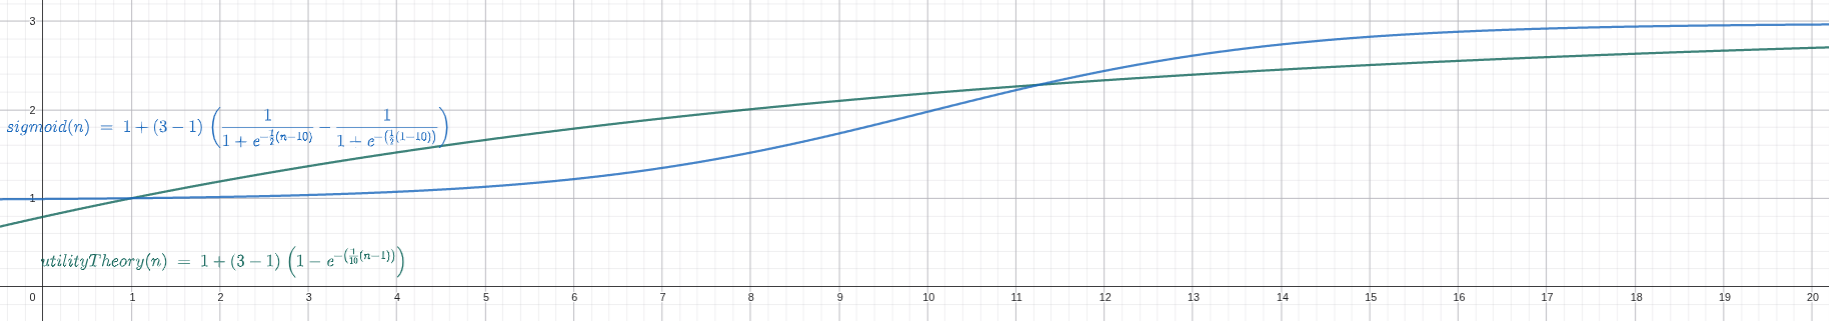
\includegraphics[width=1\textwidth]{./figures/agg_formel_vergleich.png}
    \caption{Sigmoid-Funktion und Utility-Theory-Funktion im Vergleich (X-Achse = Anzahl positiver Detektionen -1, Y-Achse = Gewichtungsfaktor).}
    \label{fig:vergleich_gewichtungsfunktionen}
\end{figure}

\subsection{Utility-Theory-Funktion}
\textbf{Asymptotische Gewichtungsfunktion:} Zur Modellierung der Relevanz wird eine Funktion gewählt, die dem Prinzip des abnehmenden Grenznutzens aus der Entscheidungstheorie folgt. 
Hierzu wird die \textit{Negative Exponential Utility Function} herangezogen, welche durch eine konstante absolute Risikoaversion (CARA) charakterisiert ist \cite[Sec.~8]{norstad1999utility}. 

Durch eine positive affine Transformation \cite[Sec.~3]{norstad1999utility} wird die Funktion so skaliert, dass sie monoton steigend gegen einen definierten Grenzwert $W_{max}$ konvergiert, wobei zusätzliche Detektionen einen abnehmenden Grenzinformationsgewinn (\textit{diminishing returns}) darstellen \cite[Sec.~1]{norstad1999utility}. 
Dies verhindert eine Verzerrung durch CTI-Reports mit extrem vielen positiven Einzeldetektionen und stellt eine robuste Aggregation sicher.

Die Gewichtung der Reports erfolgt über die folgende Funktion:
\begin{equation}
    w(n) = W_{\text{base}} + (W_{\text{max}} - W_{\text{base}}) \cdot (1 - e^{-K \cdot n})
\end{equation}

Wie die Kurve verdeutlicht, erfahren CTI-Reports mit einer steigenden Anzahl positiver Detektionen ($n$) eine kontinuierlich höhere Gewichtung ($w$). Diese konvergiert gegen einen definierten Grenzwert von $W_{\text{max}} = 3$, wodurch eine übermäßige Dominanz einzelner Berichte mit extrem hohen positiven Einzeldetektionen (Outlier) unterdrückt wird \cite[Sec.~8]{norstad1999utility}. Gleichzeitig stellt der Achsenabschnitt bei $n = 1$ sicher, dass jeder Bericht mit einem Basisgewicht von $W_{\text{base}} = 1$ in die Aggregation einfließt, um eine Mindestrelevanz aller vorliegenden Informationen zu gewährleisten.

Die praktische Umsetzung der beschriebenen Gewichtungslogik ist in Listing~\ref{lst:aggregation} (\texttt{aggregation.py}) innerhalb der Funktion \texttt{add\_report\_weight} dokumentiert.

% für geogebra:
% utilityTheory(n)=W_{base}+(W_{max}-W_{base}) (1-ℯ^(-(K (n-1))))

% sigmoid(n)=W_{base}+(W_{max}-W_{base}) (((1)/(1+ℯ^(-k (n-n_{0}))))-((1)/(1+ℯ^(-(k (1-n_{0}))))))


\subsection{Sigmoid-Funktion}

\textbf{Asymptotische Gewichtungsfunktion mit S-förmigem Verlauf:} Als Alternative zur Utility-Theory-Funktion wurde die \textit{Logistische Sigmoid-Funktion} evaluiert. Sie ist im Bereich des maschinellen Lernens weit verbreitet und findet insbesondere in neuronalen Netzen Anwendung, etwa als Aktivierungsfunktion bei der Klassifikation sowie in Graph Attention Networks zur Aggregation von Nachbarknoten \cite[Sec.~2.1]{velickovic2018gat}. Ein weiterer Vorteil des Attention based ansatztes ist das dieser eine beliebige Anzahl von Inputs verarbeiten kann \cite[Sec.~1]{velickovic2018gat}.

Durch eine positive affine Transformation sowie eine Verschiebung um den Ankerpunkt wird die Funktion so skaliert und normiert, dass bei $n = 1$ stets $w(1) = W_{\text{base}}$ gilt. Dies stellt sicher, dass jeder CTI-Report mindestens mit dem Faktor $W_{\text{base}}$ in die gewichtete Aggregation einfließt. Im Code wird $n = 1$ als Standardwert verwendet, sodass Reports ohne positive Detektionen ($n_{\text{attacks}} = 0$) mit der gewichtung = 1 bewertet werden.

Die Gewichtung der Reports erfolgt über die folgende Funktion:
\begin{equation}
    w(n) = W_{\text{base}} + (W_{\text{max}} - W_{\text{base}}) \cdot
    \left(
        \frac{1}{1 + e^{-k\,(n - n_0)}}
        -
        \frac{1}{1 + e^{-k\,(1 - n_0)}}
    \right)
    \label{eq:sigmoid_weight}
\end{equation}

Der Subtraktionsterm $\tfrac{1}{1 + e^{-k\,(1 - n_0)}}$ stellt den Ankerpunkt bei $n = 1$ sicher: Er verschiebt die gesamte Kurve vertikal so, dass $w(1) = W_{\text{base}}$ exakt erfüllt ist, unabhängig von der Wahl der Parameter $k$ und $n_0$.

Im Gegensatz zur Utility-Theory-Funktion, die rein konkav verläuft und den stärksten Anstieg bei $n = 1$ aufweist, besitzt die Sigmoid-Funktion durch den Wendepunkt bei $n_0$ einen S-förmigen Verlauf \cite[Sec.~2.1]{velickovic2018gat}. Für kleine $n < n_0$ wächst das Gewicht zunächst moderat, steigt dann steil an und flacht für $n \gg n_0$ asymptotisch gegen $W_{\text{max}}$ ab. Dies modelliert die Annahme, dass eine Mindestzahl an Detektionen überschritten werden muss, bevor ein Report als signifikant eingestuft wird.

Wie in Abbildung~\ref{fig:vergleich_gewichtungsfunktionen} zu erkennen ist, unterscheiden sich beide Funktionen vor allem im Bereich kleiner Detektionszahlen: Während die Utility-Theory-Funktion Reports mit wenigen Detektionen bereits stark gewichtet, verzögert die Sigmoid-Funktion diesen Anstieg bis zum Wendepunkt $n_0$. Für große $n$ konvergieren beide Funktionen gegen $W_{\text{max}} = 3$, wodurch die Outlier-Dämpfung in beiden Fällen strukturell garantiert ist \cite[Sec.~8]{norstad1999utility}.

Die Wahl zwischen beiden Funktionen wird im Rahmen von zukünftigen Arbeiten durch empirische Evaluierung der Aggregationsergebnisse auf realen CTI-Report-Datensätzen getroffen (siehe Kapitel~\ref{chapter:diskussion_und_forschungsluecke}).